\documentclass[12pt,openany,papersize,]{jsbook}
\usepackage[T1]{fontenc}
\usepackage[utf8]{inputenc}
\usepackage{lmodern}
\usepackage{amssymb,amsmath}
\usepackage{calc}
\usepackage[sc]{mathpazo}
\usepackage[scaled]{helvet}
\usepackage[scaled]{beramono}
\usepackage[bold]{otf}
\usepackage[final]{listings}
\usepackage[bthesis]{archlab}
% \AtBeginDvi{\special{papersize=210truemm,297truemm}}
\graphicspath{{img/}}
\usepackage{textcomp,mediabb,okumacro}
\newcommand{\figref}[1]{\textbf{図}\ref{#1}}
\newcommand{\tabref}[1]{\textbf{表}\ref{#1}}
\usepackage[final]{listings}
\lstset{                 %listingsの設定
numbers=left,            %行番号を左
numberstyle=\scriptsize, %
stepnumber=1,            %1行おきに行番号を
numbersep=1zw,           %ソースと行番号の間隔
lineskip=-0.5zw,         %行間隔 要調整
basicstyle=\ttfamily,     %ttfamily
xleftmargin=15pt,
}
\usepackage{jlisting}
%\newcommand{\unit}[1]{\ifmmode\mathrm{\,[#1]}\else $\mathrm{[#1]}$\fi}%単位に使用 数式中では空白を本文中では空白なし
\title{Research on High-speed Logic Simulation for Computer Architectures}
\authorintitle{金子~達哉}
\nendo{平成 25 年度}
\studentid{09\_06410}
\advisor{吉瀬 謙二}
\affiliation{情報工学科}
\post{准教授}

\kougai{\if0
プロセッサなどのハードウェア設計は,アーキテクチャ設計・論理設計・回路設計・物理設計といったフローで行われる.
アーキテクチャ設計と論理設計においては,RTL (Register Transfer Level) のシミュレーションが不可欠である.
このために Verilog HDL などのハードウェア記述言語が用いられることが一般的である.
\fi
\parindent=1.8em
The VLSI chips such as high performance processors or SoCs with processor elements are designed in the flow of architectural design,
logic design, circuit design, and physical design.
In the architectural design and logical design, Register Transfer Level (RTL) simulation is essential for logical verification.
Hardware description languages such as Verilog HDL or VHDL are often used for the RTL modeling and simulation.
\if0
しかし Verilog HDL によるハードウェアのシミュレーションは速度が遅く,ハードウェア設計を行う上で障害になることがあった.
\fi
But the logic simulation speed of Verilog HDL is slow.
% Because of the slow simulation speed, it is difficult to design VLSI chips.

\if0
この問題を解決することを目標に C++ 言語上で RTL モデリングを行う新しい言語である ArchHDL が提案された.
ArchHDL はハードウェアのレジスタを変数,ワイヤを関数として扱うことで,Verilog HDL に近い記述でハードウェアの論理検証を行うことができる.
\fi
ArchHDL which is a new language for hardware RTL modeling on C++ was proposed to solve this problem.
ArchHDL treats a register as a variable and a wire as a function.
The hardware description in ArchHDL is similar to that in Verilog HDL.

\if0
ArchHDL で記述したハードウェアのシミュレーションはオープンソースの Verilog シミュレータである Icarus Verilog と比較してかなり高速である.
最速な有償の Verilog シミュレータである Synopsys 社の VCS と比較しても高速であることが多い.
\fi
The architectural simulation speed with ArchHDL is much faster than
that with Icarus Verilog, which is a verilog simulator of open source.
It is often faster than VCS of Synopsys, Inc.
VCS is one of the fastest verilog simulators and proprietary software.

\if0
本論文では,ArchHDL のさらなる高速化を目指す.
(1)データ変更の有無による条件分岐の除去,(2)値を配列として格納しメモリ配置を工夫,(3)並列化という 3 つの高速化手法を提案し,実装する.
\fi
In this thesis, I aim to speed up the logical simulation with ArchHDL.
I propose and implement three methods as follows:
(1) removal of conditional branch for data update,
(2) storing register values to the continuous memory location
and (3) the parallelization of the execution of multiple instances.

\if0
マイクロベンチマークである 4096 個のカウンタ回路を用いた評価では提案手法によりオリジナルの ArchHDL と比較して 5.23 倍高速になった.
現実的なハードウェアであるステンシル計算回路を用いた評価では提案手法によりオリジナルの ArchHDL と比較して 1.95 倍高速になった.
提案手法により今回用いたすべての評価において Synopsys 社の VCS よりも高速にシミュレーションが行えるようになった.
\fi
I elapse the simulation time with 4096 of the counters circuit as a micro benchmark and a stencil-computation circuit as a realistic hardware as an evaluation.
The evaluation results as the micro benchmark show that the elapsed time of the proposed methods is 5.23 times faster than that of the original ArchHDL.
The evaluation results as the realistic hardware show that the elapsed time of the proposed methods is 1.95 times faster than that of the original ArchHDL.
The results show that ArchHDL applied the proposed methods can perform faster than VCS in the all evaluations in this thesis.
}

\setcounter{tocdepth}{3}

\title{Research on High-speed Logic Simulation \\ for Computer Architectures}
\author{金子達哉}
\date{平成 25 年 8 月}

\begin{document}
\maketitle

\frontmatter

\tableofcontents

\mainmatter

\chapter{序論(2)}

\if0
\section{研究の背景と目的}
\fi
\section{Background}

\if0
プロセッサなどのハードウェア設計は,アーキテクチャ設計・論理設計・回路設計・物理設計といったフローで行われる.
アーキテクチャ設計と論理設計においては,RTL (Register Transfer Level) のシミュレーションが不可欠である.
このために Verilog HDL などのハードウェア記述言語が用いられることが一般的である.
\fi
The VLSI chips such as high performance processors or SoCs with processor elements are designed in the flow of architectural design,
logic design, circuit design, and physical design.
In the architectural design and logical design, Register Transfer Level (RTL) simulation is essential for logical verification.
Hardware description languages such as Verilog HDL or VHDL are often used for the RTL modeling and simulation.

\if0
我々は C++ 言語上で RTL モデリングを行う新しい言語である ArchHDL を提案している~\cite{satos:archhdl}.
ArchHDL を用いることで Verilog HDL に近い記述でハードウェアの論理検証を行うことができる.
\fi
\textbf{ArchHDL} was proposed as a new language for hardware RTL modeling~\cite{satos:archhdl}.
The hardware description in ArchHDL is similar to that in Verilog HDL.

\if0
ArchHDL で記述したハードウェアのシミュレーションはオープンソースの Verilog シミュレータである Icarus Verilog~\cite{iverilog}と比較して高速である.
しかし一部のハードウェアシミュレーションにおいて有償の Verilog シミュレータである Cadence 社の NC-Verilog より高速であったが,同じく有償の Synopsys 社の VCS~\cite{vcs} より高速ではないことがあった.
しかし VCS より高速ではないことがあった.
\fi
The architectural simulation speed with ArchHDL is much faster than
that with Icarus Verilog~\cite{iverilog}, which is a verilog simulator of open source.
It is also faster than that with NC-Verilog of Cadence, Inc.
NC-Verilog is a verilog simulator and proprietary software.
However, it is not faster than that with VCS of Synopsys, Inc.~\cite{vcs} in some hardware simulation.
VCS is one of the fastest verilog simulators and proprietary software.

\if0
そこで ArchHDL に分岐の削減,メモリ配置の工夫,OpenMP による並列化といった高速化手法を適用する.
\fi
In this thesis, I aim to speed up the logical simulation with ArchHDL.
I propose and implement three fast methods as follows:
(1) removal of conditional branch for data update,
(2) storing register values to the continuous memory location
and (3) the parallelization of the execution of multiple instances.

\if0
本論文では Verilog シミュレータの Icarus Verilog, NC-Verilog, VCS と比較して,
今回の高速化手法の有用性を評価する.
Verilog シミュレータである Icarus Verilog, NC-Verilog, VCS と比較して,
今回の高速化手法の有用性を評価する.
\fi
In comparison with Icarus Verilog, NC-Verilog, and VCS which are verilog simulators, I evaluate a usefulness of fast methods in this thesis.

\if0
\section{本論文の構成}
\fi
\section{Outline of this thesis}

\if0
本論文の構成は以下の通りである.\ref{c:summary} 章で,ArchHDL の概要を述べる.
\ref{c:method} 章で,ArchHDL の高速化手法を提案する.
\ref{c:evaluation} 章で,様々な Verilog シミュレーションツールと比較して ArchHDL と今回の高速化手法の評価を行う.
\ref{c:conclusion} 章でまとめる.
\fi
The rest of this thesis is organized as follows.
Section \ref{c:summary} provides an overview of ArchHDL.
Section \ref{c:method} proposes fast methods on ArchHDL.
In section \ref{c:evaluation}, I elapse the simulation speed of ArchHDL in comparison with the various verilog simulators.
Section \ref{c:conclusion} gives the conclusion of this work.


\if0 \chapter{ハードウェア記述言語の抽象度} \fi

\chapter{ArchHDL の概要(10)}

\label{c:summary}

\if0 \#\# C++ のラムダ関数

C++11 と呼ばれる C++ ISO 標準により,ラムダ関数の仕様が定義された. gcc
では,バージョン 4.5 よりこの ISO 標準の一部がサポートされ,
標準ライブラリとしてラムダ関数が利用できるようになった.

我々の提案する ArchHDL では,このラムダ関数を利用する. ここでは,C++11
のラムダ関数の機能を ArchHDL のために必要な範囲で述べる.

\begin{figure}[t]
 \lstinputlisting[language=c++]{src/def_lam.cc.part}
 \caption{ラムダ関数の定義のみを含む C++ プログラムの例}
 \label{src:def_lambda}
\end{figure}

\figref{src:def_lambda} にラムダ関数の定義のみを含む C++
プログラムの例を示す. 2 行目のコードは引数に \verb`int x` と
\verb`int y` をとり,その和を返すラムダ関数の定義である.

ラムダ関数の定義は lambda-introducer と呼ばれる {[}{]} \footnote{
[] 内にキャプチャと呼ばれるラムダ関数の機能を指定する記述をする必要がある.
ArchHDL では [=] のみを使用するため説明は省略する.
} の記述からはじまる.ラムダ関数の返り値の型は, return
文より推測できる場合に省略できる.例に示したラムダ関数の返り値の型は int
と推測される.

\begin{figure}[t]
 \lstinputlisting[language=c++]{src/ex_lam.cc}
 \caption{ラムダ関数を定義して,それを使う C++ プログラムの例}
 \label{src:ex_lambda}
\end{figure}

\figref{src:ex_lambda} にラムダ関数を定義して,それを使う C++
のプログラムを示す. ラムダ関数を使うために,1 行目のように functional
という標準ライブラリをインクルードする.

6,7 行目で, 関数オブジェクト Sum に
\verb`[=](int x, int y) { return x + y; }` というラムダ関数を代入する.
このラムダ関数は int 型の値を返す関数であり,その型は
std::function\textless{}int ()\textgreater{} となる. これにより,Sum は
2 個の int 型の値を引数にとり,その和を返す関数オブジェクトとなる.

8 行目では Sum を呼び出し,返り値を変数 c に代入している. 引数には,4,
5 行目にある a, b を与えている.

ArchHDL では,ラムダ関数を \figref{src:ex_lambda}
のような使い方をしている.

\fi

\section{ArchHDL による RTL モデリング \label{ss:modeling}}

ArchHDL はハードウェアの RTL モデリングのための言語である.
Verilog HDL に近い記述方法を目指している.
ユーザはライブラリにより提供される Module クラス,reg クラス,wire クラスおよび C++11 のラムダ関数を用いて
ハードウェアを記述する.
\if0 ここ追加 \fi
\if0
gcc では,バージョン 4.5 より標準ライブラリとしてラムダ関数が利用できるのでこれ以上のバージョンを要求する.
\fi

\begin{figure}[t]
 \lstinputlisting[language=c++]{src/counter8.cc}
 \caption{ArchHDL による 8 ビットカウンタ回路の記述}
 \label{src:counter}
\end{figure}

\begin{figure}[t]
 \lstinputlisting[language=verilog]{src/counter8.v}
 \caption{Verilog HDL による 8 ビットカウンタ回路の記述}
 \label{src:counter_v}
\end{figure}

\figref{src:counter}に,ArchHDL を用いて記述した 8 ビットカウンタ回路のコードを示す.
また,\figref{src:counter_v} に,Verilog HDL で記述した 8 ビットカウンタ回路のコードを示す.
ArchHDL において,Module クラスを継承して定義されるクラス(Module 子クラス)は,
Verilog HDL におけるモジュールに相当する.
同様に reg クラス,wire クラスは,それぞれ Verilog HDL におけるレジスタ,ワイヤに相当する.

Module 子クラスは,そのメンバ関数として Init 関数および Always 関数を定義する必要がある.
これは,ライブラリにより強制されており,いずれかの関数が必要でない場合でも空の関数を定義する必要がある.

Init 関数には,モジュール内のすべてのワイヤへの継続代入の定義を記述する.
これは,Verilog HDL においてモジュール内で定義されている assign 文をすべてこの関数内に記述することに相当する.
wire クラスのインスタンスにラムダ関数を代入することでワイヤへの継続代入を記述することができる.
\figref{src:counter}では,6 行目で wire クラスの変数 out に reg クラス の counter の値を返す
ラムダ関数(\verb/[=]() { return counter(); }/)を代入している.
ここで,reg クラスのオブジェクトは関数として呼び出すことにより,そのサイクルにおける値を取得することができる.
このため,先のラムダ関数における counter() によってレジスタの値が取得できる.
これは,\figref{src:counter_v} の 6 行目に相当する.

Always 関数には,モジュール内のすべてのレジスタへのノン・ブロッキング代入を記述する.
ArchHDL では,単一クロックの立ち上がりエッジでの制御のみを対象としている.
これは,Verilog HDL における \verb/always @(posedge clock)/ ブロック内の記述に相当する.
reg クラスのインスタンスに \verb/<<=/ 演算子を用いて値を代入することでノン・ブロッキング代入を記述することができる.
ArchHDL は,演算子オーバーロードを利用して \verb/<<=/ 演算子を Verilog HDL における
ノン・ブロッキング代入に相当する値の代入として実装している.
\figref{src:counter}では,9 行目で reg クラスの変数 counter に自身の値をインクリメントした値を代入している.
これは,\figref{src:counter_v}の 8 行目に相当する.

ArchHDL では,データ型として C++ の整数型を使用している.
\figref{src:counter}の例では unsigned int 型を利用しているため,
8 ビットカウンタを実現するために値をマスクする必要がある.
reg クラスと wire クラスのオブジェクトは関数として呼び出すことにより,そのサイクルにおける値を取得することができる.


\if0
\section{ArchHDL の利点}

ArchHDL には,次に挙げる利点がある.

\begin{itemize}
 \item ハードウェアモジュール間の接続の記述が容易
 \item 論理シミュレーションが高速
\end{itemize}
ここでは特に重要な前者について述べる.

\begin{figure}[t]
 \centering
 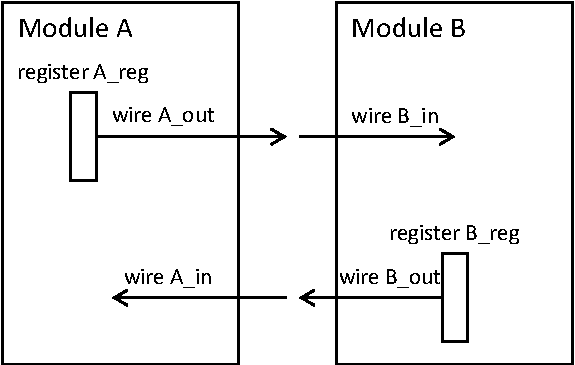
\includegraphics[clip,width=.4\textwidth]{module}
 \caption{手続き型言語では記述が難しいモジュール間の接続の例}
 \label{fig:module}
\end{figure}

\figref{fig:module} に,手続き型言語でハードウェアの挙動を記述しようとすると,
記述が難しいモジュール間の接続の例を示す.
モジュール A は入力ワイヤ A\_in,出力ワイヤ A\_out の入出力を持つ.
出力ワイヤ A\_out はレジスタ A\_reg の値を出力する.
モジュール B は入力ワイヤ B\_in,出力ワイヤ B\_out の入出力を持つ.
出力ワイヤ B\_out はレジスタ B\_reg の値を出力する.

モジュール A の出力ワイヤ A\_out は モジュール B の入力ワイヤ B\_in に接続している.
モジュール B の出力ワイヤ B\_out は モジュール A の入力ワイヤ A\_in に接続している.
モジュール A は,あるサイクルに入力として B\_reg の値を受け,A\_reg の値を出力するというモジュールである.
同様に,モジュール B は,あるサイクルに入力として A\_reg の値を受け,B\_reg の値を出力するというモジュールである.

\begin{figure}[t]
 \begin{center}
  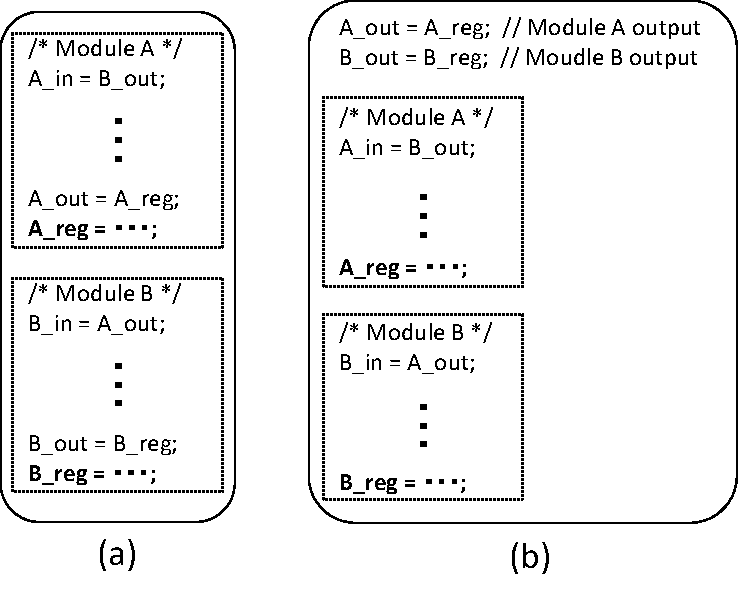
\includegraphics[width=.4\textwidth,clip]{module2}
  \caption{\figref{fig:module} のハードウェアの記述例}
  \label{fig:module2}
 \end{center}
\end{figure}

このハードウェアの挙動をモジュールごとに記述すると,\figref{fig:module2}(a)のようになる.
この記述は,
モジュールへの入力,モジュール内の処理,モジュールからの出力,レジスタの更新という
まとまりのある記述になっている.
レジスタの更新は図中の太字で示した箇所である.

手続き型言語で
\figref{fig:module2}(a)のように順番にモジュール A,モジュール B の処理が記述される場合,
モジュール A の処理の先頭にある A\_in への代入は,1 サイクル前の B\_out の状態となり,
\figref{fig:module}のハードウェアとは異なる挙動となる.

このハードウェアの挙動を手続き型言語で記述するには,
\figref{fig:module2}(b)のようにレジスタからの読み出しをモジュールごとの処理とは別に
記述するといった対策が必要である.
しかし,このような記述はモジュールが複雑になればなるほど呼び出し順序に依存関係が生じ,
保守性や可読性が損なわれる.

Verilog HDL などのハードウェア記述言語では継続代入やノン・ブロッキング代入のサポートにより
呼び出し順序に依らないハードウェアの記述が可能である.
ArchHDL では,ライブラリにより提供されるクラス群を使用してハードウェアを記述すれば,
先に例示したようなモジュールの接続も Verilog HDL 同様に記述することができる.


\section{ArchHDL の制約}

ArchHDL には,次に挙げる制約がある.

\begin{itemize}
 \item 単一クロックの立ち上がりエッジのみでレジスタの値を更新
 \item 32 ビットや 64 ビットなどの整数型をベースとした記述
\end{itemize}

実装を簡潔にするために単一クロックの同期回路で,
かつレジスタへの代入はクロックの立ち上がりエッジのみのハードウェアを対象とする.
複数のクロックや,クロックの立ち上がりエッジと立ち下がりエッジでの制御はサポートしていない.

演算に用いるデータ型として,C++ 言語の32 ビットや 64 ビットなどの整数型を使用する.
任意のビット幅のレジスタやワイヤはサポートしていない.
演算子は C++ が提供する演算子をサポートしており,
Verilog HDL で使用可能なビット切り出しやビット連結などの演算はサポートしない.


\section{テストベンチの記述}

ArchHDL は,C++ 言語をベースとしている.
したがって,ユーザは柔軟にテストベンチを記述することが可能である.
ここでは,ArchHDL の提供するライブラリを用いたテストベンチ記述の一例を示す.

\begin{figure}[t]
 \lstinputlisting[language=c++]{src/cnt_testtop.cc}
 \caption{ArchHDL を用いたカウンタ回路のためのテストベンチの記述例}
 \label{src:test}
\end{figure}

\figref{src:test} は,先に示したカウンタ回路の ArchHDL によるテストベンチの記述例である.
インクルードの記述などは省略している.また,14 行目と 16行目の HALT\_CYCLE は定数である.

このテストベンチ記述は,テストモジュール TestTop を作成し,
その中でカウンタ回路のインスタンスを生成しテストを行うという設計になっている.
そのために,22 行目からの main 関数は簡潔になり,TestTop モジュールのインスタンス生成と
ライブラリによりステップ実行のみの記述となる.

ArchHDL は,モジュールのインスタンスを生成する際にすべての reg クラスのインスタンス,
wire クラスのインスタンスをライブラリで一元管理する設計になっている.
そのため,23 行目のようにモジュールのインスタンスを生成したのち,
ArchHDL により提供される Step 関数(25行目)を呼び出せばサイクルごとのシミュレーションができる.

\begin{figure}[t]
 \lstinputlisting[language=verilog]{src/cnt_testtop.v}
 \caption{Verilog HDL を用いたカウンタ回路のためのテストベンチの記述例}
 \label{src:test_v}
\end{figure}

\figref{src:test} に挙げたテストベンチの記述は,Verilog HDL で同様の記述ができるという利点がある.
\figref{src:test_v} に Verilog HDL を用いて同様のテストベンチを記述する例を示す.
ArchHDL を用いた場合と大きく異なる点は 14 行目においてクロックを生成している部分である.
それ以外の記述については ArchHDL と Verilog HDL で大きな違いはない.

\fi

\section{ArchHDL の実装} \label{ss:implementation}

ArchHDL のライブラリには,Module クラス,wire クラス,reg クラス,これらの 3 個のクラスのインタフェースクラス,
Singleton クラスの 7 個のクラスが定義されている.
本章では,標準ライブラリのインクルードをのぞくすべてのライブラリのコードを示しながら ArchHDL の実装について述べる.
以降の説明では,ユーザが Module クラスを継承して作成したクラスを Module 子クラスと呼ぶ.

\begin{figure}[p]
  \lstinputlisting[language=c++,basicstyle=\ttfamily\footnotesize]{src/singleton.cc}
 \caption{ArchHDL ライブラリにおける各インタフェースクラスと Singleton クラスと Step 関数の定義}
 \label{src:class_singleton}
\end{figure}

\figref{src:class_singleton} に RegisterInterface クラス,ModuleInterface クラス,WireInterface クラス,
Singleton クラスおよび Step 関数の定義を示す.

ModuleInterface クラス,WireInterface クラス,RegisterInterface クラスは
それぞれ Module クラス,wire クラス,reg クラスのインタフェースクラスである.
Singleton クラスが,Module 子クラス,wire クラス,reg クラスのインスタンスを
シングルトン・パターンにより一元管理する.
これは,ArchHDL のライブラリにおいて核となるクラスである.

Singleton クラスは,メンバ変数として Module クラス,wire クラス,reg クラスの
インタフェースクラスのポインタを格納する可変行列をもつ(18 ~ 20 行目).
Module 子クラス,wire クラス,reg クラスのインスタンスが生成される際に,
そのインスタンスへのポインタが Singleton クラスに渡される.
また,ポインタは Singleton クラスに渡される際にそれぞれのインタフェースクラスに自動でアップキャストされる
(26 ~ 34 行目).

Step 関数(50 ~ 57 行目)は,1 サイクルのシミュレーションを行う関数である.
Step 関数を呼び出すと,Singleton クラスの Exec 関数が呼ばれる.
ただし,初回 Step 関数の呼び出しのみ Singleton クラスの Init 関数が呼ばれる.
Step 関数を繰り返し呼び出すことにより,複数サイクルにわたるシミュレーションが行なわれる.

Init 関数(35 ~ 39 行目)は,保持しているすべての Module 子クラスのインスタンスの Init 関数を呼ぶ(37 行目).
%これにより,ユーザが Module 子クラス内に定義したワイヤの継続代入の処理が行われる.

Exec 関数(40 ~ 47 行目)は,保持しているすべての Module 子クラスのインスタンスの Always 関数を呼び(42 行目),
次に保持しているすべての reg クラスのインスタンスの Update 関数を呼ぶ(45 行目).

Always 関数によりすべてのレジスタについて次のサイクルにおける値が計算される.
Update 関数によりレジスタの値が更新される.
この Always と Update の処理によりレジスタのノン・ブロッキング代入を実現する.


\subsection{reg クラスの定義}

\begin{figure}[tp]
 \lstinputlisting[language=c++]{src/reg.cc}
 \caption{ArchHDL ライブラリにおける reg クラスの定義}
 \label{src:reg}
\end{figure}

\figref{src:reg} に,reg クラスの定義を示す.
reg クラスは,扱うデータ型をテンプレート引数にとるテンプレートクラスである.
また,インタフェースクラスである RegiterInterface クラスを継承する.

ArchHDL ではレジスタを変数として扱うため,
reg クラスはメンバ変数にテンプレート引数で与えられたデータ型の変数 curr\_ と next\_ を持つ(5,6 行目).
curr\_ は,あるサイクルにおけるレジスタの値で,next\_はその次のサイクルのレジスタの値である.
Module 子クラスの Always 関数の呼び出しにより,next\_に値が代入される.
reg クラスのメンバ関数 Update を呼ぶことで,next\_ の値は curr\_ に反映される(15 ~ 20 行目).
これによりレジスタへのノン・ブロッキング代入の挙動を実現する.

reg クラスのオブジェクトへの値の代入をそのメンバ変数 next\_ への値の代入とするために,
演算子オーバーロードにより \verb`<<=` 演算子を再定義している(24 ~ 27 行目).
\verb`<<=` 演算子により代入された値は,変数 next\_ に格納され,set\_ フラグがセットされる.

ArchHDL では,
すべての Module 子クラスのインスタンスの Always 関数を呼び出した後に,
すべての reg クラスのインスタンス Update 関数を呼び出す.
したがって,Always 関数が呼び出されている間に取得できる
レジスタの値 curr\_ は Update 関数が呼ばれるまで保持されている.

reg クラスのコンストラクタ(12 ~ 14 行目)では,
メンバ変数を初期化し,自身のポインタを Singleton クラスに渡す処理が行われる.
テスト記述や初期値設定のために = 演算子による値の代入も定義されている(21 ~ 23 行目).
= 演算子による値の代入は,式が評価された時点で curr\_ の値を変更する.
reg クラスのインスタンスを関数として呼び出すことで curr\_の値を取得することができる(28 ~ 29 行目).


\subsection{wire クラスの定義}

\begin{figure}[t]
 \lstinputlisting[language=c++]{src/wire.cc}
 \caption{ArchHDL ライブラリにおける wire クラスの定義}
 \label{src:wire}
\end{figure}

\figref{src:wire} に,wire クラスの定義を示す.
wire クラスは,テンプレート引数として扱うデータ型をとるテンプレートクラスである.
また,インタフェースクラスの WireInterface クラスを継承している.

ArchHDL では,ワイヤは関数として扱うため,
wire クラスはメンバ変数にラムダ関数 lambda\_ を持つ(4 行目)クラスとなっている.
このラムダ関数は,テンプレート引数として与えられたデータ型を返す関数である.

コピーコンストラクタの禁止(7,8 行目)と演算子のオーバーロード(13,14 行目)により,
wire クラスへの = 演算子による代入はラムダ関数に限定される.
これにより,wire クラスのオブジェクトは Module 子クラスの Init 関数で記述される
ラムダ関数を保持するクラスとなる.

wire クラスのコンストラクタ(10 ~ 12 行目)では,
メンバ変数を初期化し,自身のポインタを Singleton クラスに渡す処理が行われる.
wire クラスのオブジェクトを関数として呼び出すと,
自身の持つラムダ関数を呼び出した結果を返す(16 ~ 18 行目).
これにより,wire クラスのオブジェクトを関数呼び出しすることで,
そのサイクルでのワイヤの値が取得できる.

\subsection{Module クラスの定義}

\begin{figure}[t]
 \lstinputlisting[language=c++]{src/module.cc}
 \caption{ArchHDL ライブラリにおける Module クラスの定義}
 \label{src:module}
\end{figure}

\figref{src:module} に,Module クラスの定義を示す.
Module クラスは,インタフェースクラスの ModuleInterface クラスを継承するクラスである.
ArchHDL でハードウェアを記述する際に,このクラスを継承してモジュールを記述する.

コンストラクタ(7 ~ 9行目)では,自身のポインタを Singleton クラスに渡す.
ModuleInterface クラスにおいて Init 関数と Always 関数が仮想関数として定義されているため,
これらの関数を定義する必要がある.
Module クラスは,Module 子クラスのインタフェースとして定義しているため,
Init 関数と Always 関数として空の関数を定義している(10,11 行目).


\if0

\section{ArchHDL の性能解析 \label{ss:profiling}}

ArchHDL の高速化に向けて性能解析を行う.
各メソッドの実行にどの程度時間を要しているかを調べる.
性能解析には gprof~\cite{gprof}を利用する.

\begin{table}[t]
 \caption{ステンシル計算回路での性能解析の結果.実行時間に占める割合が大きい 3 つの関数を示した.}
 \label{table:stencil_prof}
 \begin{center}
  % \setlength{\tabcolsep}{3pt}
  \begin{tabular}{l|r} \hline
  関数名 & 実行時間に占める割合 (\%) \\ \hline
  reg::Update() & 24.21 \\
  ArchHDL::Step() & 11.09 \\
  brk & 10.72 \\ \hline
  \end{tabular}
 \end{center}
\end{table}

\begin{table}[t]
 \caption{ステンシル計算回路でのメソッド呼び出し回数結果}
 \label{table:stencil_method_call_count}
 \begin{center}
  % \setlength{\tabcolsep}{3pt}
  \begin{tabular}{l|r} \hline
  関数名 & 実行回数 \\ \hline
  ArchHDL::Step()   &     328,425 \\
  reg::Update()     & 325,469,175 \\
  Module::Always()  &  43,680,525 \\ \hline
  \end{tabular}
 \end{center}
\end{table}

\tabref{table:stencil_prof} にステンシル計算回路での性能解析の結果を示す.
実行時間に占める割合の大きかった上位 3 つを示した.
これらの関数が全実行時間に占める割合は 46.02\% である.
これらのメソッドの実行時間の割合はそれぞれ排他的である.

最も実行時間の割合が大きい reg::Update() はインスタンスメソッドなので全インスタンスでの実行時間の合計である.
brk はデータセグメントのサイズを変更する関数である.

このように ArchHDL は,ArchHDL::Step() と reg::Update()
の実行時間が全体の実行時間に占める割合が非常に大きい.よって
ArchHDL::Step() と reg::Update() の実行を高速化することを \ref{s:method}
章で考える.

\tabref{table:stencil_method_call_count}
はステンシル計算回路でのそれぞれのメソッド呼び出し回数である.Module::Always()
はユーザが定義するので ArchHDL
側で高速化が出来る余地はない.よってそれ以外の ArchHDL::Step() と
reg::Update() の実行を高速にする.

\fi

\chapter{ArchHDL の高速化手法の提案と実装(8)}

\label{c:method}

\section{最適化の方針}

最適化の方針として逐次プログラミングにおける最適化と並列化における最適化の両方を考える.

\section{逐次プログラムにおける高速化手法}

\subsection{データ変更の有無による条件分岐の除去 \label{sss:no_set}}

\figref{src:reg} に示した実装では,reg クラスのインスタンスの値を更新する方法としてブロッキング代入とノン・ブロッキング代入の 2 つが存在する.

ブロッキング代入について考える.reg クラスのインスタンスにブロッキング代入が行われた時に curr\_ の値を書き換える.

一方でノン・ブロッキング代入について考える.
reg クラスのインスタンスにノン・ブロッキング代入が行われた時にメンバ変数 set\_ を true にし,メンバ変数 next\_ に値を代入する.
そして reg::Update 内では set\_ が true の時だけ next\_ をメンバ変数 curr\_ に代入する.
これは reg クラスのインスタンスの値を変更したサイクルのみで,
その reg クラスのインスタンスの値を次サイクルに移る前に新しい値に更新することを意味する.

\figref{src:reg} に示した実装では,
更新されない reg クラスのインスタンスの curr\_ と next\_ の値が同じであるため,代入する処理を行う必要はない.
よって set\_ 変数を用いて不要な代入を避けている.
reg クラスのインスタンスの更新頻度が低い回路であればこの実装が効率的である.

提案手法について述べる.
この set\_ 変数が true の時のみ代入するのではなく,
次サイクルに移る前に next\_ の値を curr\_ に常に代入するようにする.
こうすることによって分岐のオーバーヘッドが無くなるため,ノン・ブロッキング代入が頻繁に行われる回路で速度向上が期待できる.

\subsection{値を配列として格納しメモリ配置を工夫} \label{sss:mem_copy}

\begin{figure}[t]
 \centering
 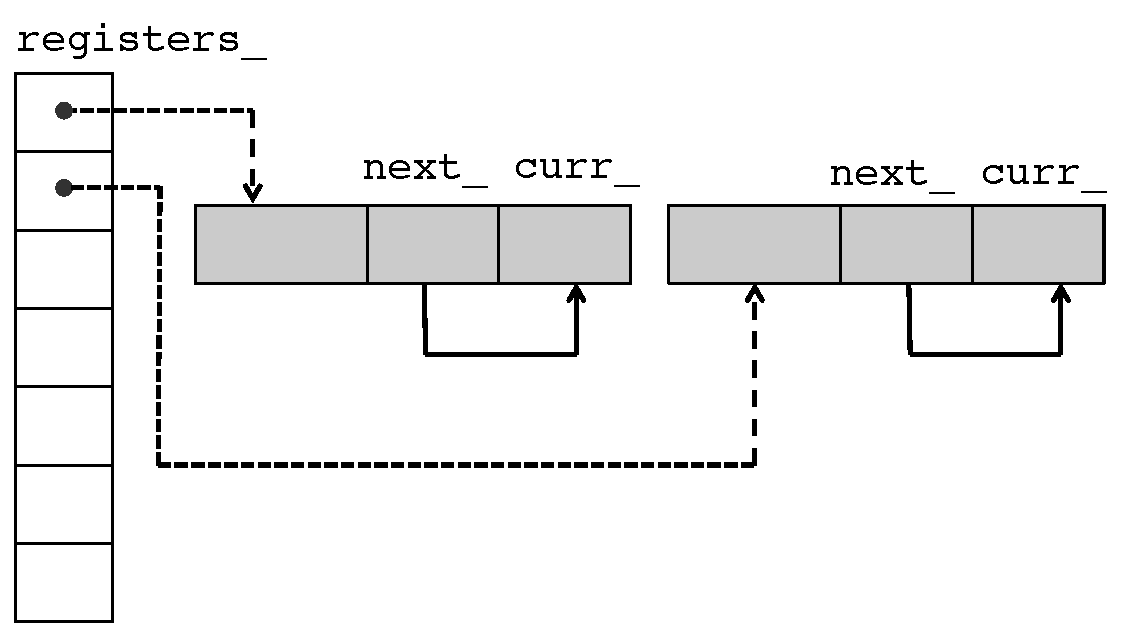
\includegraphics[clip,width=\linewidth-30pt]{registers_orig}
 \caption{ArchHDL における reg クラスのインスタンスの処理の様子}
 \label{fig:regs}
\end{figure}

\figref{fig:regs} は ArchHDL における reg クラスのインスタンスの処理の様子である.
\figref{src:class_singleton} の 44 行から 46 行の処理を表している.
reg クラスのインスタンスが灰色に塗られており,左からクラスのメタデータ,next\_, curr\_ を表している.
左側の大きな枠が\figref{src:class_singleton} の 18 行の \verb`std::vector` 型の registers\_ である.
実線矢印は代入を表し.点線矢印はポインタ参照を表す.

ArchHDL ではノン・ブロッキング代入をシミュレーションするために registers\_ の値を上から順に辿り,
reg クラスの各インスタンスのポインタを取得する.
そして reg クラスの全インスタンスの reg::Update() メソッドを呼ぶ.

\ref{sss:no_set} 節で述べたデータ変更の有無による条件分岐の除去を行うと reg::Update() メソッド内で行なっている
reg クラスのインスタンスの curr\_ に next\_ の値を代入する処理は
毎サイクル全 reg クラスのインスタンスで実行されることになる.

この代入する処理と reg::Update() メソッドの関数呼び出しの 2 つのオーバーヘッドが ArchHDL の高速化を妨げている.

\begin{figure}[t]
 \centering
 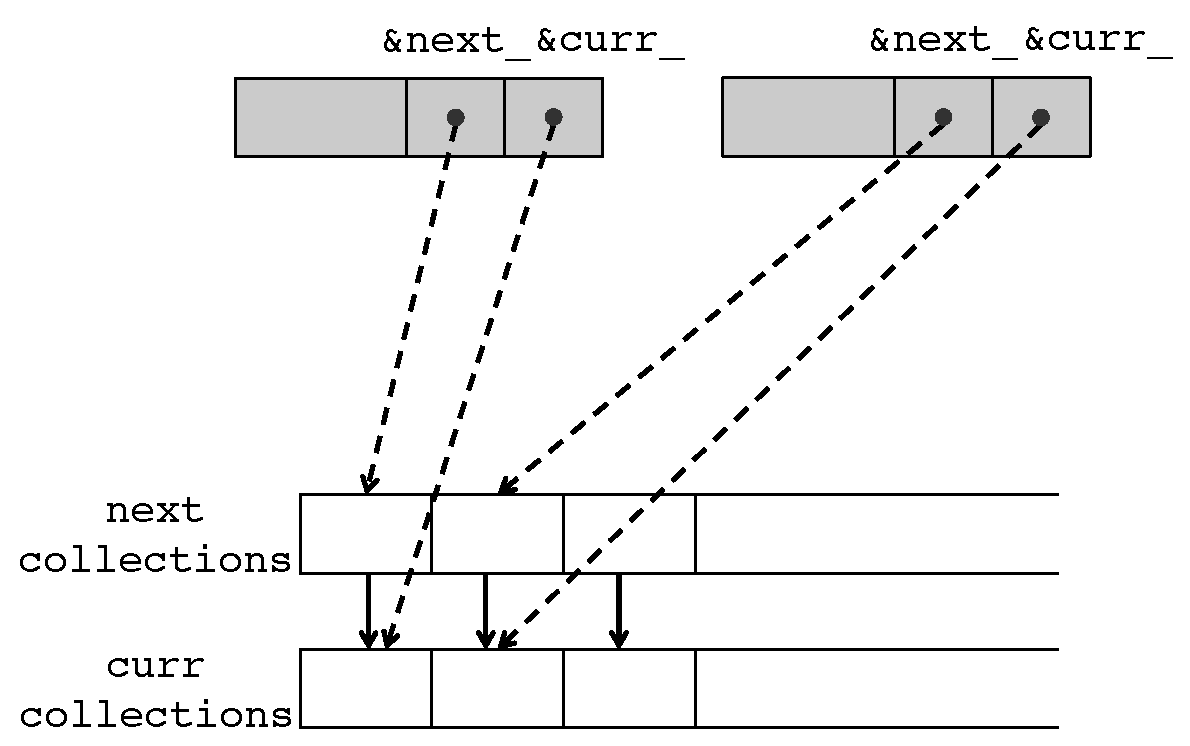
\includegraphics[clip,width=\linewidth-30pt]{registers_mem}
 \caption{値を配列として格納しメモリ配置を工夫した reg クラスのインスタンスの処理の様子}
 \label{fig:mem_copy}
\end{figure}

提案手法について述べる.
\figref{fig:mem_copy} に値を配列として格納しメモリ配置を工夫した reg クラスのインスタンスの処理の様子を示す.
\figref{fig:mem_copy} は提案手法である.
提案手法では全 reg クラスのインスタンスは現在の値と次サイクルの値の実体は持たず,ポインタを保持するように変更している.
reg クラスのインスタンスが灰色に塗られており,左からクラスのメタデータ,\&next\_, \&curr\_ を表している.
\&next\_, \&curr\_ は next\_, curr\_ のポインタである.
下の枠が next\_, curr\_ の値をまとめた配列であり,
ここでは next collections, curr collections と呼ぶ.
実線矢印は代入を表し,点線矢印はポインタの参照先を表す.

ArchHDL の実装では次サイクルに移る前に行われる curr\_ に next\_ の値を代入する処理は
reg クラスのインスタンスが存在するアドレスを調べる必要がある.
しかし値を配列として格納しメモリ配置を工夫すると\figref{fig:mem_copy} に示すように単純な代入となる.
また今まで飛び飛びのアドレスに格納されていた next\_ と curr\_ のメモリ配置がまとまるのでメモリアクセスが連続的に行える.
さらに reg::Update() の関数呼び出しが不要となり,関数呼び出しのオーバーヘッドもなくなる.
これらの理由により高速化が期待できる.

提案手法の実装について述べる.
next collections, curr collections として 2 つの十分大きな \verb/unsigned int/ 型の配列を用意する.
記述された型に応じて,reg クラスのコンストラクタが next\_, curr\_ それぞれの領域を next collections, curr collections に確保する.
確保する領域は参照の高速化のために 4 バイトの倍数とする.
確保された next\_ と curr\_ のアドレスを取得し,インスタンス内の \&next\_, \&curr\_ がそれを保持する.
これまで reg クラスの全インスタンスの reg::Update() メソッドを呼び出していたところを next\_ collections から curr\_ collections の値コピーに変更する.


\if0
\subsection{ダブルバッファリング}

これまでの実装では \ref{ss:implementation} 章で述べたように
reg クラスのインスタンスの次サイクルの値が次サイクルに移る前に reg クラスのインスタンスの現在の値に代入される.
そこで偶数回目の実行と奇数回目の実行で次サイクルの値と現在の値を格納している変数をを入れ替えれば
(ダブルバッファリング)代入が減ることが期待できる.

\begin{figure}[t]
 \begin{center}
  \input{img/reg_curr_next}
 \end{center}
 \caption{reg クラスのインスタンスの変数保持の処理の様子}
 \label{fig:reg_curr_next}
\end{figure}

\begin{figure}[t]
 \begin{center}
  \input{img/double_buffer2}
 \end{center}
 \caption{ダブルバッファリングの処理の様子}
 \label{fig:double_buffer}
\end{figure}

\figref{fig:reg_curr_next} はこれまでの ArchHDL の reg クラスのインスタンスの値の保持のイメージである.
読み込み用と書き込み用の変数をそれぞれ保持している.
読み込み用が現在の値であり,書き込み用が次サイクルの値である,
次サイクルに移る前に書き込み用の値が読み込み用の変数に書き込まれる.

\figref{fig:double_buffer}
はダブルバッファリングのイメージである.
奇数回目のサイクルと偶数回目のサイクルで読み込み用と書き込み用の変数を入れ替える.
これにより奇数回目のサイクルで書き込み用であった変数には値が書き込まれているので次サイクルの偶数回目のサイクルで読み込み用として使用出来る.
これを繰り返すことで,次サイクルに移る前に行われる代入処理を無くせる.

しかし今回の手法では reg クラスのインスタンスへ値の書き込みが行われなかった場合に
reg クラスのインスタンスのその時の書き込み用の値に更新が入らない.
次サイクルではその書き込み用の値がそのまま現在の値として使用されるので古い値が使われてしまう.
そのため単純に入れ替えるだけの実装では誤ったシミュレーションを行なってしまう.

また今回の手法はサイクルの回数で依存関係が発生するので \ref{ss:parallel} 節で述べる並列化ができない.

よってライブラリの実装として導入するのは困難であるが,
reg クラスのインスタンスへ常に書き込みが行われるカウンタ回路で試したところ効果があった(具体的な数字).
常に reg クラスのインスタンスに書き込みが行われるハードウェアシミュレーションを逐次処理で行いたい場合には高い効果が期待できる.

以上の理由から本論文ではダブルバッファリングによる評価は行わない.

\fi

\section{並列化による高速化} \label{ss:parallel}

これまで逐次実行による高速化を考えてきたが,本節では並列化による高速化について考える.

\figref{src:class_singleton} の 40 行〜 47 行に示すように
毎サイクル,Module クラスと reg クラスの全インスタンスの Module::Always() メソッドと reg::Update() メソッドが呼び出されている.

\figref{src:class_singleton} の41行〜43行で実行される Module::Always() メソッドはユーザが自由に記述できる.
そのため各 Module クラスのインスタンスで独立に Module::Always() メソッドが実行できる保証はない.
しかしここでは独立に実行できると仮定する.
独立に実行できる条件は今後の研究課題とする.
この場合 \figref{src:class_singleton} の41行〜43行に示している Module::Always() メソッドの実行は並列化が可能である.

\figref{src:class_singleton} の 44 行〜 46 行で行われるレジスタの更新は\figref{fig:regs} の実線で表されている.
各インスタンスで独立に行えるので並列化が可能である.

\figref{src:class_singleton} の41行〜47行に示している Module クラスと reg クラスの全インスタンスの Module::Always() メソッドと reg::Update() メソッドの実行は並列化が可能である.
提案手法について述べる.よってこの部分を並列化する.並列化には OpenMP~\cite{openmp} を用いる.

\begin{figure}[t]
 \lstinputlisting[language=c++]{src/exec_openmp.cc}
 \caption{Exec メソッド内の for 文を OpenMP で並列化したプログラム}
 \label{src:exec_openmp}
\end{figure}

\figref{src:exec_openmp} は\figref{src:class_singleton} の 40 行〜 47 行が 8 スレッドで並列化が行われるように OpenMP 指示文を与えたソースコードである.
2 行目は並列化を何スレッドで行うかを与えている.
今回は 8 をスレッド数に指定している.この数字は環境によって変えることができる.
4 行目と 8 行目は for 文の実行を並列化する OpenMP 指示文である.

一般に,並列化を行う場合は各スレッドに対して均等に負荷を与えることが重要である.
OpenMP では for 文の負荷を分散するスケジュール方法として,静的に決定する static や,動的に決定する dynamic など複数の方法が存在する.
一般に,スケジュール方法に dynamic を指定した場合,各スレッドに割り当てられる負荷が均等に近くなるメリットはあるが,オーバーヘッドが大きいデメリットがある.
よって ArchHDL により記述されたハードウェア記述では各モジュールと各レジスタの負荷が大幅に変わらないのであれば,static を指定した方が効率が良いと考えられる.

他にも OpenMP にはオプションとしてチャンクサイズを指定できる.
スケジュール方法を static にし,チャンクサイズを指定しなければ,チャンクサイズはループの反復数をスレッド数で割った商とほぼ同じ値になる.

今回の評価ではスケジュール方法は static でチャンクサイズは指定しないデフォルトの設定で行う.


\chapter{評価(10)}

\label{c:evaluation}

\if0
本章では ArchHDL での論理シミュレーションの実行時間を評価し,Icarus Verilog, NC-Verilog, VCS での論理シミュレーションの実行時間と比較する.
\fi
In this chapter, I evaluate the elapsed time of logic simulation in ArchHDL and it is compared with that of logic simulation in Icarus Verilog, NC-Verilog and VCS.

\begin{table}[t]
\if0
 \caption{実行環境}
\fi
 \caption{Simulation environment}
 \label{table:exec_env}
 \begin{center}
  \begin{tabular}{l|c|c} \hline
         &  Icarus Verilog, ArchHDL  &  NC-Verilog, VCS   \\ \hline
  OS     &  Ubuntu12.04             &  CentOS5.9        \\
  CPU    &  Core i7-3770K 3.50GHz   &  Core i7-3770K 3.50GHz  \\
\if0
  メモリ  &  $16\,\mathrm{GB}$       &  $16\,\mathrm{GB}$  \\ \hline
\fi
   Memory &  $16\,\mathrm{GB}$       &  $16\,\mathrm{GB}$  \\ \hline
  \end{tabular}
 \end{center}
\end{table}

\if0
\tabref{table:exec_env} に実行環境をまとめる.
評価には同じ仕様の 2 台の計算機を用いる.
一台は Icarus Verilog, ArchHDL の評価に用いる.もう一台は NC-Verilog, VCS の評価に用いる.
CPU,メモリなどのハードウェアの仕様は同一であるがソフトウェアの制約により異なる OS を利用する.
\fi
\tabref{table:exec_env} shows the simulation environment.
I use the two computers of the same specification for the evaluation.
I use to evaluate Icarus Verilog and ArchHDL
One computer is used to elapse the simulation time with Icarus Verilog and ArchHDL.
The other is used to elapse that with NC-Verilog and VCS.
The two computers are the same specification such as hardware, CPU, memory and so on.
However, I use different operating systems due to the limitations of the software.

\if0
異なる OS を用いる理由を述べる.
NC-Verilog と VCS は RedHat 系のディストリビューションのみをサポートしている.
今回は RedHat 系のディストリビューションである CentOS5.9 を用いる.
しかし CentOS5.9 に含まれる gcc のバージョンは 4.1.2 である.
\ref{s:lambda}節で述べたように,ArchHDL では C++11 のラムダ関数を用いて記述するため gcc のバージョンは 4.5 以上が必要である.
その条件を満たす Ubuntu12.04 を評価に用いる.
Ubuntu12.04 に含まれる gcc のバージョンは 4.6.3 である.
gcc の最適化オプションとして \verb/-O2/ を用いる.
Icarus Verilog はどちらのディストリビューションでも動作するが,今回は Ubuntu12.04 を用いる.
Ubuntu12.04 に含まれる Icarus Verilog のバージョンは 0.9.5 である.
VCS のバージョンは vcsC-2009.06 を用いる.NC-Verilog のバージョンは 06.20-s004 を用いる.
\fi
I describe the reason for using different operating systems.
NC-Verilog and VCS support only RPM-based Linux distributions.
I use CentOS5.9 which is RPM-based Linux distributions for this evaluation.
However, the version of GCC includes CentOS5.9 is 4.1.2.
I describe it in Section \ref{s:lambda} that the version of GCC requires 4.5 or greater for using the lambda function in ArchHDL.
I also use to evaluate the Ubuntu12.04 satisfying the condition.
The version of GCC includes Ubuntu12.04 is 4.6.3.
I use \verb/-O2/ as optimization option of GCC.
Icarus Verilog runs on both computers.
I use it on Ubuntu12.04 in this evaluation.
The version of Icarus Verilog includes Ubuntu12.04 is 0.9.5.
The version of NC-Verilog is 06.20-s004.
The version of VCS is vcsC-2009.06.

\if0
今回用いる計算機の CPU の物理コアは 4 コアであるため, OpenMP による並列化はスレッド数を 8 個にして評価する.
\fi
Because physical cores of the CPU of the computers are 4 cores for this evaluation,
I evaluate the parallelization with OpenMP in 8 threads

\if0
評価では,2 つのマイクロベンチマークと,現実的なハードウェアのベンチマークとしてステンシル計算回路\cite{koba:stencil}を用いる.
Verilog HDL と ArchHDL のためのハードウェアシミュレーションは手作業により作成した.
両ハードウェアシミュレーションの出力は同様になるように作成した.
\fi
In the evaluation, I use two micro benchmarks
and stencil-computation circuit as a benchmark of hardware realistic.
I have created hardware simulation for ArchHDL and Verilog HDL by myself
and the output of both the hardware simulation to be same.

\if0
評価結果に用いているラベルの名前について述べる.
オリジナルの ArchHDL は \textbf{ArchHDL} と表す.
\ref{sss:no_set} 節で述べた条件分岐の除去を適用したものを \textbf{NO SET} と表す.
\ref{sss:mem_copy} 節で述べたメモリ配置の工夫を適用したものを \textbf{MEM MAP} と表す.
\ref{ss:parallel} 節で述べた並列化を行ったものを \textbf{PARA} と表す.
メモリ配置の工夫と並列を同時に適用したものを \textbf{MEM MAP + PARA} と表す.
\fi
I describe the name of the labels which are used on the evaluation results.
Original ArchHDL is named \textbf{ArchHDL}.
It is named \textbf{NO SET} that I apply removal of the conditional branch to ArchHDL, which is described in Section \ref{sss:no_set}.
It is named \textbf{MEM MAP} that I apply devising a memory allocation and stored as an array to ArchHDL, which is described in Section \ref{sss:mem_copy}
It is named \textbf{PARA} that I apply the parallelization to ArchHDL, which is described in Section \ref{ss:parallel}.


\section{Evaluation by Micro Benchmark}

\if0
マイクロベンチマークとしてカウンタ回路と XORSHIFT による乱数生成回路を用いる.
\fi
I elapse the simulation time with the counter circuits and the random number generator circuits by XORSHIFT RNG as micro benchmarks.

\begin{figure}[tb]
 \lstinputlisting[language=c++]{src/xorshift_alg.cc}
\if0
 \caption{XORSHIFT 法に基づく乱数生成のアルゴリズム}
\fi
 \caption{The algorithm of random number generation based on XORSHIFT RNG on C language}
 \label{src:xorshift_alg}
\end{figure}

\if0
カウンタ回路とは \figref{src:counter} に示した 1 サイクルごとに 1 を足す回路である.
ハードウェアの規模を増やすためにカウンタの数を指定できるようにした.
XORSHIFT による乱数生成回路とはシフトと XOR 演算のみで構成できる XORSHIFT 法に基づく乱数生成器をハードウェア記述によって実装した回路である.
\figref{src:xorshift_alg} に XORSHIFT 法に基づく乱数生成のアルゴリズムを C 言語によって実装したものを示す.
\fi
The counter circuit is a circuit that adds 1 per cycle as shown in \figref{src:counter}.
I can specify the number of the counter in order to increase the scale of hardware.
The random number generator circuits by XORSHIFT RNG is a circuit which is implemented as the random number generator based on XORSHIFT RNG by a hardware description.
XORSHIFT RNG use only the \textit{exclusive or} and a \textit{bit shifted} to generate the random numbers.
\figref{src:xorshift_alg} shows the algorithm of random number generator based on XORSHIFT RNG on C language.

\begin{figure}[tb]
 \centering
 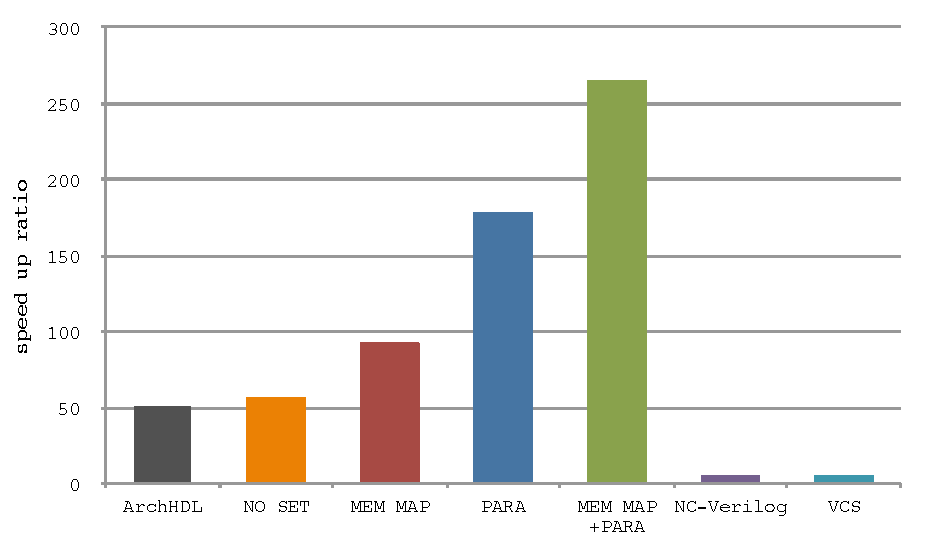
\includegraphics[clip,width=\linewidth]{counter_4096}
\if0
 \caption{4096 個のカウンタ回路の実行時間を Icarus Verilog と比較した速度向上比}
\fi
 \caption{Speed up ratio compared with the elapsed time of 4096 of the counter circuit with Icarus Verilog}
 \label{fig:counter4096}
\end{figure}

\if0
\figref{fig:counter4096} に 4096 個のカウンタ回路の実行時間を Icarus Verilog と比較した速度向上比を示す.
縦軸は Icarus Verilog での実行時間を 1 とした速度向上比を示している.
\fi
\figref{fig:counter4096} shows speed up ratio compared with the elapsed time of 4096 of the counter circuit with Icarus Verilog.
The Speedup ratio as elapsed time in Icarus Verilog is 1 is denoted in the vertical axis.

\if0
ArchHDL は商用の NC-Verilog, VCS と比較してもかなり高速である.
\textbf{MEM MAP + PARA} の論理シミュレーション実行時間は NC-Verilog の 58.8 倍,VCS の 56.7 倍高速である.
\fi
The simulation time of ArchHDL is much faster that that of NC-Verilog and VCS.
The evaluation result shows that the elapsed time of \textbf{MEM MAP + PARA} is 58.8 times faster than that of NC-Verilog and 56.7 times faster than that of VCS.

\if0
また今回提案している高速化手法はオリジナルの ArchHDL に比べていずれも効果が出ている.
\textbf{MEM MAP + PARA} の論理シミュレーション実行時間はオリジナルの ArchHDL の 5.23 倍高速である.
\fi
The proposed methods in this paper are effective as compared with the original ArchHDL.
The elapsed time of \textbf{MEM MAP + PARA} is 5.23 times faster than that of the original ArchHDL.



\begin{figure}[tb]
 \centering
 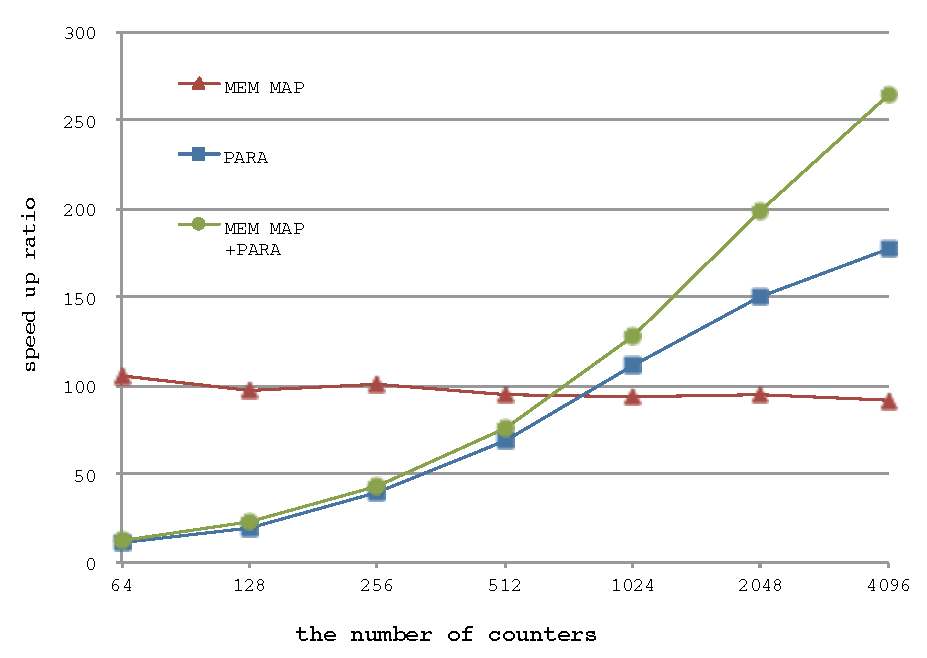
\includegraphics[clip,width=\linewidth]{counter_con}
\if0
 \caption{高速化手法を適用した ArchHDL と OpenMP を適用したカウンタ回路の実行時間を Icarus Verilog と比較した速度向上比}
\fi
 \caption{Speed up ratio compared with the elapsed time of the counter circuits with Icarus Verilog in ArchHDL applying the fast method and OpenMP}
 \label{fig:counter_con}
\end{figure}

\if0
\figref{fig:counter_con} に高速化手法を適用した ArchHDL と OpenMP を適用したカウンタ回路の実行時間を Icarus Verilog と比較した速度向上比を示す.
縦軸は Icarus Verilog での実行時間を 1 とした速度向上比を示している.
横軸はカウンタの個数である.
\fi
\figref{fig:counter_con} shows speed up ratio compared with the elapsed time of the counter circuits with Icarus Verilog in ArchHDL applying the fast method and OpenMP.
The Speedup ratio as elapsed time in Icarus Verilog is 1 is denoted in the vertical axis.
The number of counters is denoted in horizontal axis.

\if0
\textbf{MEM MAP} は逐次に実行されているので Icarus Verilog と比較した速度向上比はカウンタの個数を変えてもほとんど変わらない.
並列化を行った \textbf{PARA} と \textbf{MEM MAP + PARA} はカウンタの個数が 1024 個以上で \textbf{MEM MAP} よりも高速になる.
\textbf{PARA} より \textbf{MEM MAP + PARA} の方が常に高速であるので今回提案している逐次処理での高速化手法は並列化を行った場合でも効果が出ている.
カウンタの個数はハードウェアの規模とみなせるため,並列化が有効なのはある程度規模の大きい回路であると言える.
\fi
Speed up ratio compared to Icarus Verilog is almost unchanged if you change the number of the counters because \textbf{MEM MAP} is executed in sequential program.
The elapsed time of \textbf{PARA} and \textbf{MEM MAP + PARA} which are executed in parallel is faster than that of \textbf{MEM MAP} if the number of counters is 1024 or more.
The proposed methods in sequential program are effective in parallel
because the simulation time of \textbf{MEM MAP + PARA} is always faster than that of \textbf{PARA}.
Because the number of counters can be regarded as the scale of hardware, the parallelization is effective if the hardware is large-scale.


\begin{figure}[tb]
 \centering
 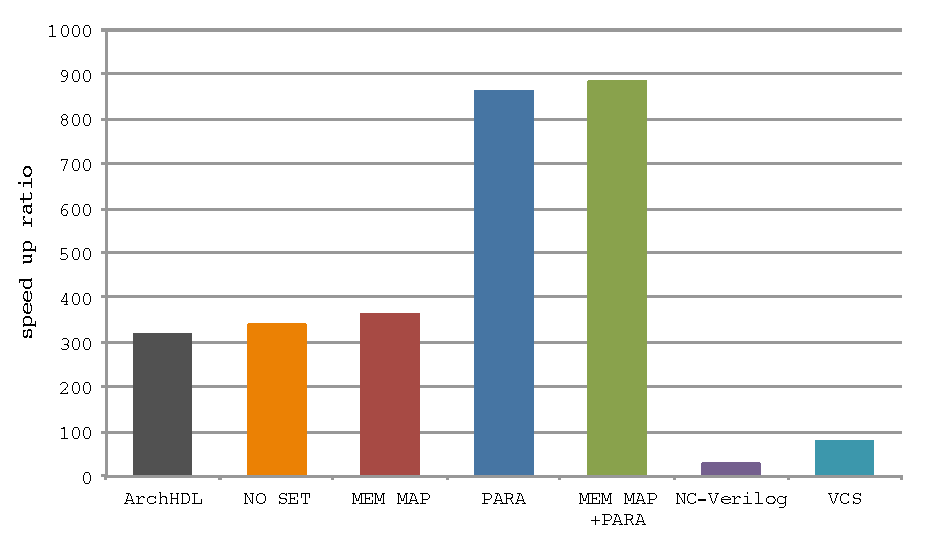
\includegraphics[clip,width=\linewidth]{xorshift}
\if0
 \caption{512 個の XORSHIFT による乱数生成器の実行時間を Icarus Verilog と比較した速度向上比}
\fi
 \caption{Speed up ratio compared with the elapsed time of 512 of the random number generator circuits by XORSHIFT RNG with Icarus Verilog}
 \label{fig:xorshift}
\end{figure}

\if0
\figref{fig:xorshift} は XORSHIFT による乱数生成器での実行時間を Icarus Verilog と比較した速度向上比である.
試行回数は 524,288 回である.初期値の異なる乱数生成器を 512 個用意している.
\fi
\figref{fig:xorshift} shows speed up ratio compared with the elapsed time of 512 of the random number generator circuits by XORSHIFT RNG with Icarus Verilog.
The number of trials is 524,288 times.
I use the 512 random number generators with different initial values.

\if0
ArchHDL は商用の NC-Verilog, VCS と比較してもかなり高速である.
\textbf{MEM MAP + PARA} の論理シミュレーション実行時間は NC-Verilog の 32.2 倍,VCS の 11.3 倍高速である.
\fi
The simulation time of ArchHDL is much faster than that of NC-Verilog and VCS.
The simulation time of \textbf{MEM MAP + PARA} is 32.2 times faster than that of NC-Verilog and 11.3 times faster than that of VCS.

\if0
また今回提案している高速化手法はオリジナルの ArchHDL に比べていずれも効果が出ている.
\textbf{MEM MAP + PARA} の論理シミュレーション実行時間はオリジナルの ArchHDL の 2.78 倍高速である.
\fi
The proposed methods in this paper are effective as compared with the original ArchHDL.
The simulation time of \textbf{MEM MAP + PARA} is 2.78 times faster than that of the original ArchHDL.


\section{Evaluation by Stencil-Computation Circuit}

\if0

\begin{table}[tb]
 \caption{ステンシル計算回路でのプロファイリング結果 1.1}
 \label{table:stencil_prof1.1}
 \begin{center}
  % \setlength{\tabcolsep}{3pt}
  \begin{tabular}{lr} \toprule
  関数名 & 実行時間に占める割合 (\%) \\ \midrule
  reg::Update() (合計) & 16.57 \\
  ArchHDL::Step() & 12.47 \\
  brk & 15.05 \\ \bottomrule
  \end{tabular}
 \end{center}
\end{table}

\fi

\begin{figure}[tb]
 \centering
 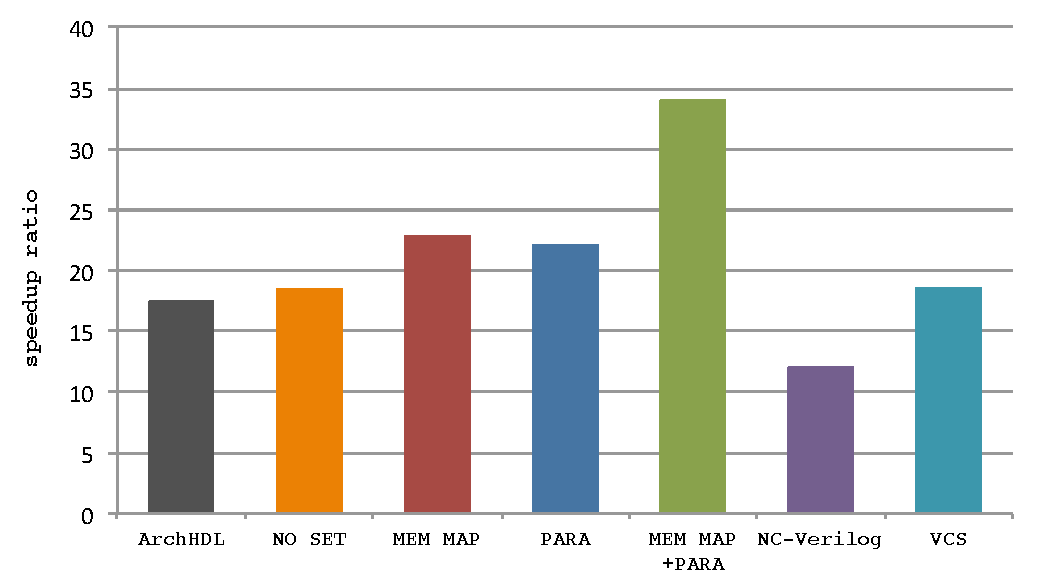
\includegraphics[clip,width=\linewidth]{stencil}
\if0
 \caption{ステンシル計算回路の Icarus Verilog と比較した実行時間の速度向上比}
\fi
 \caption{Speed up ratio compared with the elapsed time of a stencil-computation circuit with Icarus Verilog}
 \label{fig:stencil}
\end{figure}

\if0
\figref{fig:stencil} はステンシル計算回路での実行結果である.
縦軸は Icarus Verilog と比較したそれぞれの速度向上比である.
\fi
\figref{fig:stencil} shows speed up ratio compared with the elapsed time of a stencil-computation circuit with Icarus Verilog.
The Speedup ratio as elapsed time in Icarus Verilog is 1 is denoted in the vertical axis.

\if0
オリジナルの ArchHDL は商用の NC-Verilog より高速であったが,同じく商用の VCS はオリジナルの ArchHDL と \textbf{NO SET} より高速である.
しかし逐次実行での高速化手法と並列化を共に適用した \textbf{MEM MAP + PARA} の論理シミュレーション実行時間は VCS の 1.83 倍高速である.
\fi
The simulation time of the original ArchHDL is faster than that of NC-Verilog.
The simulation time of the original ArchHDL and \textbf{NO SET} is not faster than that of VCS.
But the simulation time of \textbf{MEM MAP + PARA} is 1.83 times faster than that of VCS.

\if0
ステンシル計算回路の場合は Update() は 325,469,175 回呼ばれているのに対して,
reg の値に更新がないのは 5,145,760 回である.
つまり更新がないのは Update() メソッド呼び出し全体の $1.58\%$ 程度に過ぎない.
それにより条件分岐を無くす \textbf{NO SET} の論理シミュレーションはオリジナルの ArchHDL より高速である.
また Update() のメソッド呼び出しを減らし,かつメモリ配置を工夫している \textbf{MEM MAP} の論理シミュレーション実行時間はオリジナルの ArchHDL の 1.31 倍高速である.
\fi
\textit{Update} method is called 325,469,175 times in a stencil-computation circuit.
The number of the value of the reg updated is 5,145,760 times.
That is, the number of the value of the reg not updated is not only $1.58\%$ of the entire \textit{Update} method call.
Therefore the simulation time of \textbf{NO SET} is faster than that of the original ArchHDL.
The simulation time of \textbf{MEM MAP} is 1.31 times faster than that of the original ArchHDL.

\if0
また Module が 133 個,reg が 991 個存在する回路なので並列化の効果も大きい.
逐次実行での高速化手法と並列化を共に適用した \textbf{MEM MAP + PARA} の論理シミュレーション実行時間はオリジナルの ArchHDL の 1.95 倍高速である.
\fi
The parallelization is effective because this hardware with ArchHDL has the 133 \textit{Module} class instance and the 991 \textit{reg} class instance.
The simulation time of \textbf{MEM MAP + PARA} is 1.95 times faster than that of the original ArchHDL.


% \subsection{高速化の解析}


\chapter{結論(2)}

\label{c:conclusion}

ハードウェアの RTL モデリングのための新しい言語として提案している ArchHDL の高速化手法を提案し,実装し,評価した.
ArchHDL ではハードウェアのレジスタを変数,ワイヤを関数として扱うことで,C++ で RTL モデリングを実現する.

高速化手法として (1)データ変更の有無による条件分岐の除去,(2)値を配列として格納しメモリ配置を工夫,
(3)並列化手法を提案した.

提案手法を実装し,ArchHDL を Icarus Verilog と商用ツールである VCS, NC-Verilog の実行時間と比較した.
マイクロベンチマークである 4096 個のカウンタ回路を用いた評価では提案手法によりオリジナルの ArchHDL と比較して 5.23 倍高速になった.
現実的なハードウェアであるステンシル計算回路を用いた評価では提案手法によりオリジナルの ArchHDL と比較して 1.95 倍高速になった.
提案手法により今回用いたすべての評価において Synopsys 社の VCS よりも高速にシミュレーションが行えるようになった.


\backmatter

\chapter{謝辞}

\label{c:acknowledgment}

研究を進めるにあたり.適切な指導をしていただいた指導教員の吉瀬謙二准教授に感謝します.吉瀬研究室の皆様にも数々の助言をいただき,大変お世話になりました.特に吉瀬研究室の博士課程の佐藤真平さんには多大な貢献をしていただきました.また同じく博士課程の高前田(山崎)伸也さんと笹河良介さんにも数多くの助言をしていただきました.

入谷優さんにも論文の構成など数多くの助言をしていただきました.

ArchHDL の開発に多大な貢献をしていただいた佐野伸太郎さんに感謝します.


\label{c:relatedwork}

\def\newblock{\hskip .11em plus.33em minus.07em}
\bibliographystyle{ipsjunsrt}
\bibliography{thesis,standards,url}


\end{document}
